% SC4063 --- Chapter 3: Intrusion Detection and Prevention (0->100)
\chapter{Intrusion Detection and Prevention}\label{ch:ids}
\sloppy

\begin{quote}
\emph{``Firewalls decide who may pass; IDS decides who already passed and
looks guilty.''} --- One enforces a guest list, the other watches the crowd.
\end{quote}

\noindent\fbox{\parbox{\dimexpr\linewidth-2\fboxsep-2\fboxrule}{%
\textbf{From zero: seeing is a system.} We start from a single packet copy,
ask what to compare it against (a signature or a model of normal), then build
the pipeline that turns copies into alerts and, optionally, into drops. No IDS
background assumed; every component is motivated before it is named.}}
\vspace{0.4em}

\section*{Learning Outcomes}
After this chapter you will be able to:
\begin{enumerate}[label=(L\arabic*)]
    \item contrast NIDS, NIPS, and HIDS placement and fail-open vs.\ fail-closed;
    \item distinguish signature, anomaly, and hybrid detection and their ROC trade-offs;
    \item author and tune Snort/Suricata rules and suppress false positives;
    \item explain base-rate fallacy, evasion, and encrypted-traffic limits;
    \item correlate alerts via SIEM and argue IDS vs.\ IPS blocking policy.
\end{enumerate}

% ============================================================
\section{Where the Sensor Sits}\label{sec:placement}
A firewall is inline by definition; an IDS may be passive (copy) or inline
(block). The vantage determines risk.

\begin{definition}[NIDS vs.\ NIPS vs.\ HIDS]\label{def:nids}
A \emph{NIDS} copies traffic via SPAN/mirror or TAP, raises alerts, never
blocks. A \emph{NIPS} is inline and can drop, reset, or quarantine; every
NIPS is a NIDS that also enforces. A \emph{HIDS} runs on the host and sees
syscalls, logs, and file integrity. Network sees the wire; host sees the
outcome.
\end{definition}

\begin{figure}[h]\centering
\begin{tikzpicture}[scale=0.82, every node/.style={font=\scriptsize},
  box/.style={draw,thick,rounded corners=4pt,minimum width=2.35cm,minimum height=0.95cm,align=center}]
\node[box,fill=red!12] (inet) at (0,1.90) {Internet};
\node[box,fill=orange!15] (fw) at (3.0,1.90) {Firewall};
\node[box,fill=blue!14] (tap) at (3.0,0.40) {NIDS\\\tiny SPAN/TAP (copy)};
\node[box,fill=green!15] (lan) at (6.2,1.90) {LAN / servers};
\node[box,fill=violet!12] (host) at (6.2,0.40) {HIDS\\\tiny host agent};
% inline NIPS as diamond gate between fw and lan
\node[draw,thick,fill=red!18,diamond,aspect=1.7,inner sep=2pt,minimum width=1.45cm] (ips) at (4.65,1.90) {NIPS};
\draw[->,thick] (inet) -- (fw);
\draw[->,thick] (fw) -- (ips);
\draw[->,thick] (ips) -- (lan) node[midway,above,font=\tiny] {inline, may drop};
\draw[->,thick,dashed,blue!60!black] (fw) -- (tap) node[midway,left,font=\tiny] {mirror};
\draw[->,thick,dashed,violet!60!black] (lan) -- (host);
\node[font=\tiny,fill=yellow!12,rounded corners=2pt,inner sep=2pt,draw=gray!40] at (3.0,-0.55) {NIDS is fail-open (tap fails $\to$ traffic still flows)};
\node[font=\tiny,fill=red!12,rounded corners=2pt,inner sep=2pt] at (6.2,-0.55) {NIPS is fail-closed or fail-open by policy};
\end{tikzpicture}
\caption{Sensor placement. NIDS taps a copy; NIPS sits inline as a gate; HIDS watches the host. Colour distinguishes passive (blue/violet) from enforcing (red/orange).}
\label{fig:placement}
\end{figure}

Inline placement creates a failure-mode choice. \emph{Fail-open}: if the NIPS
crashes, traffic passes uninspected (availability over security). \emph{Fail-
closed}: traffic stops (security over availability). Data centres choose fail-
open for revenue; safety-critical networks choose fail-closed.

Modern EDR/XDR fuses all three: network metadata plus host telemetry in one
timeline. Encrypted traffic blinds the network sensor, pushing visibility to
the endpoint or to a TLS-intercept proxy with explicit consent.

% ============================================================
\section{What to Compare Against}\label{sec:detection}
Two philosophies compete: look for the known bad, or model the known good.

\begin{description}[leftmargin=1.2em,itemsep=0.35em]
    \item[Signature-based] Matches known patterns: byte sequences, regex on
    headers/payload, or Snort rules.
    \texttt{alert tcp any any -> any 80 (msg:"SQLi"; content:"' OR 1=1";)}
    has low false positives but is blind to zero-days and needs frequent
    updates. Analogous to antivirus signatures. Snort (single-threaded) and
    Suricata (multi-threaded, YAML config) dominate open source.
    \item[Anomaly-based] Learns a model of normal (traffic volume, n-gram
    entropy, host behaviour) and flags deviation beyond a threshold. Catches
    novel attacks; suffers higher false positives and adversarial mimicry
    (attacker shapes traffic to look normal). Needs clean training data.
    \item[Hybrid] Signature for the known, anomaly for the unknown, with a
    correlation layer (SIEM) to combine. Production default.
\end{description}

\begin{figure}[h]\centering
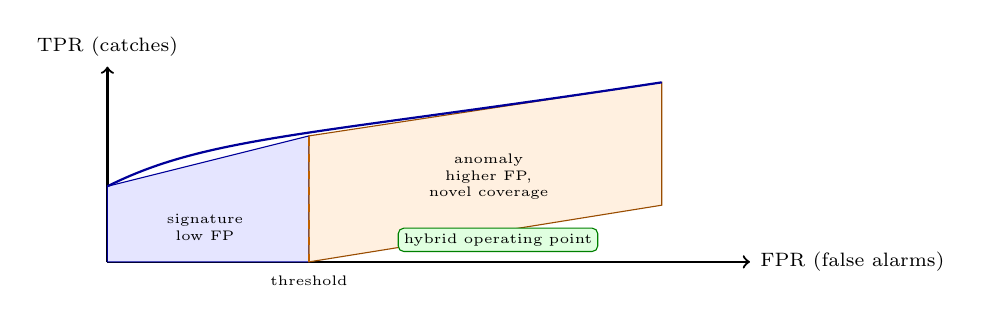
\begin{tikzpicture}[scale=0.80, every node/.style={font=\scriptsize}]
\draw[->,thick] (0,0) -- (10.2,0) node[right] {FPR (false alarms)};
\draw[->,thick] (0,0) -- (0,3.1) node[above] {TPR (catches)};
\fill[blue!10,draw=blue!60!black] (0,0) -- (3.2,0) -- (3.2,2.0) -- (0,1.2) -- cycle;
\fill[orange!12,draw=orange!60!black] (3.2,2.0) -- (8.8,2.85) -- (8.8,0.90) -- (3.2,0) -- cycle;
\draw[thick,blue!60!black] (0,1.2) .. controls (1.6,2.0) and (3.2,2.0) .. (8.8,2.85);
\draw[thick,orange!75!black,dashed] (3.2,0) -- (3.2,2.0);
\node[font=\tiny,align=center] at (1.55,0.55) {signature\\\tiny low FP};
\node[font=\tiny,align=center] at (6.05,1.35) {anomaly\\\tiny higher FP,\\novel coverage};
\node[font=\tiny,fill=green!12,rounded corners=2pt,inner sep=2pt,draw=green!50!black] at (6.2,0.35) {hybrid operating point};
\node[font=\tiny] at (3.2,-0.30) {threshold};
\end{tikzpicture}
\caption{ROC intuition. Signatures sit at low FPR with a ceiling; anomaly pushes the curve outward at higher FPR. Operators choose a threshold per response (block vs.\ alert).}
\label{fig:roc}
\end{figure}

Metrics: true/false positives/negatives, ROC curve, and the \emph{base-rate
fallacy}: even 1\% FPR on 1\,M daily events with 10 true attacks yields
$\approx$10\,000 alerts and precision 0.1\%. That is why signatures dominate
inline blocking (low FP required) while anomaly is often alert-only for a SOC
analyst.

\begin{figure}[h]\centering
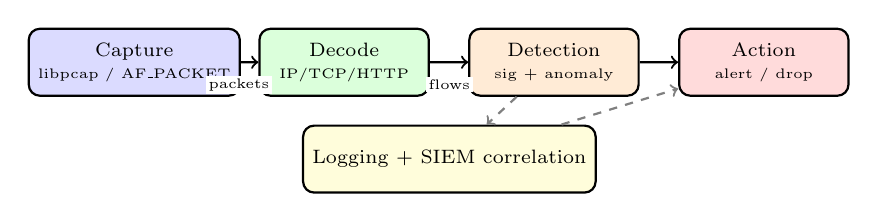
\begin{tikzpicture}[scale=0.82, every node/.style={font=\scriptsize},
  idsbox/.style={draw,thick,rounded corners=4pt,minimum width=2.15cm,minimum height=0.85cm,align=center}]
\node[idsbox,fill=blue!14] (cap) at (0,1.20) {Capture\\\tiny libpcap / AF\_PACKET};
\node[idsbox,fill=green!14] (dec) at (3.25,1.20) {Decode\\\tiny IP/TCP/HTTP};
\node[idsbox,fill=orange!16] (det) at (6.50,1.20) {Detection\\\tiny sig + anomaly};
\node[idsbox,fill=red!14] (act) at (9.75,1.20) {Action\\\tiny alert / drop};
\draw[->,thick] (cap) -- (dec); \draw[->,thick] (dec) -- (det); \draw[->,thick] (det) -- (act);
\node[idsbox,fill=yellow!14,minimum width=3.0cm] (log) at (4.88,-0.30) {Logging + SIEM correlation};
\draw[->,thick,dashed,gray] (det) -- (log); \draw[->,thick,dashed,gray] (log) -- (act);
\node[font=\tiny,fill=white,inner sep=1pt] at (1.62,0.85) {packets};
\node[font=\tiny,fill=white,inner sep=1pt] at (4.88,0.85) {flows};
\end{tikzpicture}
\caption{IDS pipeline. Every stage can be tuned: capture performance (AF\_PACKET, DPDK), decode coverage, detection thresholds, and action policy.}
\label{fig:ids-pipeline}
\end{figure}

\begin{lstlisting}[language=Python,caption={Toy IDS: signature match + entropy anomaly sketch.},label={lst:ids-toy}]
import re, math, collections
RULES = [re.compile(p) for p in [r"' OR 1=1", r"<script", r"\.\./"]]
def inspect(payload: str):
    for r in RULES:
        if r.search(payload):
            return f"ALERT sig:{r.pattern!r}"
    return "OK"
# Anomaly: byte entropy deviates >2 sigma from baseline
baseline = (4.2, 0.6)  # mean, stdev of entropy for normal HTTP payloads
def entropy(s): 
    from collections import Counter
    c = Counter(s.encode()); n = len(s) or 1
    return -sum((v/n)*math.log2(v/n) for v in c.values())
def anomaly(payload):
    e = entropy(payload)
    return abs(e-baseline[0]) > 2*baseline[1]
print(inspect("GET /?q=' OR 1=1 --"))  # ALERT sig
print(anomaly("A"*800 + "\x00\xff"*20))  # True if entropy odd
\end{lstlisting}

\begin{lstlisting}[language=bash,caption={Suricata rule and tuning snippet.},label={lst:suricata}]
# /etc/suricata/rules/local.rules  -- signature
alert http any any -> any any (msg:"SQLi UNION SELECT"; \
  http.uri; content:"UNION"; nocase; content:"SELECT"; distance:0; \
  classtype:web-application-attack; sid:1000001; rev:1;)
# suricata.yaml -- suppress a noisy false positive for a known scanner
# threshold: type suppress, track by_src, ip 10.0.2.15, sid 1000001
\end{lstlisting}

Tuning is the job: suppress noisy SIDs, add flowbits to correlate across
packets, and write threshold rules (\texttt{5 hits in 10s}) to turn probes
into incidents. Without tuning, an IDS becomes an alert firehose that hides
real compromise.

Evasion reminds us detection is adversarial. Attackers fragment packets, vary
case, encode payloads, or tunnel over encryption so the NIDS never sees the
bytes the endpoint reassembles. Normalisation (reassemble before matching) and
endpoint visibility are the counters; they cost CPU and are never perfect.

\begin{remark}[Encrypted traffic]\label{rem:encrypt}
TLS blinds payload inspection. Options: (a) inspect at the endpoint (HIDS),
(b) decrypt at a forward proxy with consent and re-encrypt (enterprise
TLS inspection, privacy trade-off), or (c) detect on metadata (flow sizes,
timing, JA3 fingerprints, DNS). Choice is policy, not just technology.
\end{remark}

% ============================================================
\section{Exercises}\label{sec:ch03-exercises}
\begin{enumerate}[label=E3.\arabic*, leftmargin=*, itemsep=0.6em]
    \item \textbf{Placement.} A 10\,Gbps link carries trading traffic.
    Argue for NIDS vs.\ NIPS, fail-open vs.\ fail-closed, and where you would
    also need HIDS. What does encryption do to your choice?
    \item \textbf{ROC arithmetic.} A signature set has 1\% FPR on 1\,M daily
    events with 10 true attacks. Compute expected alerts and precision. An
    anomaly detector catches 9/10 at 5\% FPR. Compute its alerts and say which
    is suitable for inline blocking vs.\ SOC monitoring.
    \item \textbf{Rule authoring.} Write a Suricata rule that alerts on
    \texttt{../../etc/passwd} in \texttt{http.uri} (case-insensitive) and add a
    \texttt{threshold} to alert only if seen 3 times from the same source in 60s.
    Explain how to suppress it for a scanner at \texttt{10.0.2.15}.
    \item \textbf{Base-rate intuition.} Even with 99\% TPR and 1\% FPR, why does a
    base rate of 1 attack in 100\,000 flows make most alerts false? Compute
    posterior probability of a true attack given an alert (Bayes).
    \item \textbf{Evasion.} Show two distinct ways to evade a naive
    \texttt{content:"cmd.exe"} NIDS signature without changing the endpoint's
    behaviour (fragmentation, encoding, case, etc.). Propose a normalisation
    that defeats each.
\end{enumerate}

\section*{Chapter Notes}
IDS taxonomy is Denning (1987) and Axelsson (2000); Snort (Roesch, 1999) and
Suricata (OISF, 2010) exemplify signatures. Sommer--Paxson (2010) critiques
anomaly hype; fraud-base-rate analysis follows Axelsson. Evasion via insertion
and fragmentation is Ptacek--Newsham (1998). SIEM correlation and encrypted-
traffic visibility are covered in NIST SP~800-94 (IDS/IPS) and SP~800-83
(malware/EDR). Zeek (formerly Bro) is the canonical network monitor for
metadata-first detection.
% End of Chapter 3
